\documentclass[11pt]{article}
\usepackage{fullpage}
%\usepackage{soul}
\usepackage{bm,amsmath,amssymb}
\usepackage{custom_style}
\usepackage{graphicx}
\usepackage[linesnumbered, ruled]{algorithm2e}
\usepackage{hyperref}
\usepackage{color}
\usepackage{url}
%\usepackage{natbib}
\usepackage{array}
\definecolor{mydarkblue}{rgb}{0,0.08,0.45}
\hypersetup{ % play with the different link colors here
	colorlinks,
	citecolor=mydarkblue,
	filecolor=mydarkblue,
	linkcolor=mydarkblue,
	urlcolor=mydarkblue % set to black to prevent printing blue links
}

\newcommand{\mname}{\texttt{Med2Vec}\xspace}
\newcommand{\argmax}{\operatornamewithlimits{argmax}}
\newcommand{\argmin}{\operatornamewithlimits{argmin}}

\begin{document}
	
	\title{\textbf{Convolutional Neural Network (CNN) based Model for\\
			 Patient Representation Learning to Uncover Temporal\\ Phenotypes for Heart Failure}%
		\date{}
		%\date{July 9, 2014}
		\author{
			Chongchao Zhao$^1$ \quad Yichen Shen$^2$ \quad Li-Pan Yao$^1$\\
			$^1$ MS Analytics, Georgia Institute of Technology\\
			$^2$ MS Computer Science, Georgia Institute of Technology
		} %
	}

	
	\maketitle
	\begin{abstract}
		Electronic Health Records (EHR) are immense datasets filled with a wealth of all kinds of medical data for each patient for each medical visit. However, traditional methods of data analysis on EHR datasets prove impenetrable due to its size, dimensionality, and irregularity. Heart failure (HF) has frustrated caregivers due to its nature as an overarching condition rather than a distinct phenotype. For instance, there are two proposed broad phenotypes of HF based on reduced or preserved ejection fraction; while one phenotype is quite treatable, the other phenotype is difficult to treat. In this work, we propose to utilize convolutional neural networks (CNN) on EHR data pre-processed by Word2Vec, which would allow us to efficiently extract informative representations of HF patients. The representation can help identify a new set of phenotypes with similar EHR profiles to facilitate treatment of patients with HF.
	\end{abstract}
	
	% The code below should be generated by the tool at
	% http://dl.acm.org/ccs.cfm
	% Please copy and paste the code instead of the example below. 
	%
	
	
	\section{Introduction}
	\label{sec:intro}
	%\input{intro.tex}
	\paragraph{}
	Currently, there are about 5.7 million adults in the United States suffering from heart failure (HF). HF has contributed around 1/9 of the deaths per year, and about half of the patients die within 5 years of diagnosis [Mozaffarian 2016]. Furthermore, HF costs the nation an estimated \$30.7 billion each year [Heidenreich 2011]. Due to the high morbidity and mortality, an increasing prevalence, and the escalating healthcare costs associated with HF, there is ongoing effort in clinical research to identify high-risk patients in order to provide more precise prediction and apply customized treatment [Alba 2013]. Such predictions include differentiating HF patients with the reduced ejection fraction (rEF) phenotype which has ample effective treatments from the patients with preserved ejection fraction (pEF) which currently has no effective treatment options [Lindman 2017, Austin 2013].
	
	Among the various efforts to this end, the data mining approach became increasingly popular. In the context of the complexity and vast volume of healthcare transactions, which are difficult to process with more traditional analytical methods, modern data mining techniques such as advanced machine learning and the more recent deep-learning methods have particular merits. Through utilizing health information technology (HIT) infrastructure in the form of electronic health records (EHRs), many aspects of care including diagnosis, medication, laboratory results and imaging data could be captured [Jensen 2012].  Extracting meaningful representation of various groups of similar patients from electronic records, sometimes called computational phenotyping, would have a wide range of beneficial impact on facilitating clinical research in HF as well as in other areas in health care.
	
	However, mining useful information in EHR remains extremely challenging. The electronic record data are usually complex, high-dimensional, noisy, incomplete, and longitudinally irregular. Currently, Existing EHR driven studies in HF or other areas often rely on carefully engineered features chosen by domain experts [Smith 2011, Taslimitehrani 2016].  However, there are a couple of limitations to such analyses. First, these types of feature engineering require a lot of domain knowledge and are sometimes costly and difficult to generalize. Second, the context and temporal relationship between different features are ignored in the setting of traditional HF research, which can sometimes contain crucial information to identify risk groups.
	
	To cope with these limitations, we utilize deep learning learning method to efficiently extract robust patient representation for HF risk prediction from EHR without manual feature engineering. The concept of our model is inspired by the Word2Vec model [Mikolov 2013] and Convolutional Neural Networks (CNN) in the context of natural language processing (NLP) [Kim 2014]. Specifically, via the Word2Vec model, single patient events are transformed to distributed embedding forms that contain hidden semantic relationships between different medical events. We can then utilize a CNN model taking in a sequence of patient events and predict the risk of HF. Owing to its special convolutional operation, CNN model can automatically learn latent structure in sequential relationships between events. Combining those two models we are able to extract the context and temporal relations in patient-level medical events from EHR and provide robust patient representation pertaining to HF risk prediction. 
	
	Since deep learning applications in clinical studies is still in its nascency, there are only a few papers that incorporated deep learning in EHR driven studies. Some previous research has highlighted the efficacy of the application of CNN and Word2Vec to EHR-driven prediction tasks [Che 2017, Nguyen 2016]. We extend their work and provide some interpretation of patient-level representation learned by CNN in HF prediction.
	
	
	\section{Methodology}
	\label{sec:method}
	%\input{method.tex}
	
	\subsection{Feature Embedding Learning via Word2Vec}
	
	\paragraph{}Since its publication in 2013, word2vec, developed by Google, has gained much popularity in multiple areas such as NLP and deep learning. It takes a text corpus as input and outputs word vectors. Learned representations are based on distance which calculates the similarity between words. It does not require labels, and with enough training data, the resulting word vectors have embeddings with intriguing characteristics in such a manner that words with similar meanings appear in clusters.
	
	EHRs are essentially time-series comprising sequences of encounter episodes. For a given patient, we observe his/her events in a temporal order. For MIMIC-III dataset, we focus on diagnoses, procedures and prescriptions. In the context of word2vec, we extract the information of ICD9 codes, procedure items, and drug names from a patient’s medical record and arrange these words into a sequence which can be likened to a “sentence”. Then word2vec is used to train this collection of sentences. As a result, each word in a sentence representing a patient will be converted to an array. These arrays could then be stacked to become a matrix which can be fed into a CNN.
	
	However, this process assumes the intervals of hospital visit are uniformly distributed. To capture the heterogeneity of intervals, we add an interval tag to the records. For example, if time difference between two consecutive codes is ~3 months, we add a tag ‘2-4m’ between them. We have discretized the observation window into several intervals associated with different tags. 
	
	\subsection{CNN Risk Prediction Model}
	
	\paragraph{}Convolutional Neural Networks (CNN) is efficient in extracting underlying local structures. It has been widely used in computer vision and speech recognition area and achieved significant success.  It’s more recent application in NLP  and video processing demonstrates its capability of extracting temporal and sequential information [Kim 2014, Karpathy 2014]. Hence, in temporally ordered EHR data, CNN is very suitable for mining hidden structure and local dependencies for each patient’s records that are useful for predicting diseases.
	
	Specifically, we construct input for given patient $p$ as a embedding matrix $X_p \in R^{n_p * d}$, where $n_p$ is the number of records the patient have in the observation window and $d$ is the dimension of embedding for each patient’s medication records, diagnosis records, and input tags. Note that the records are ordered temporally and the temporal dimension of of the matrix $n_p$ varies across different patients. We then apply 1D convolutional operation over temporal dimensions of the matrix. Suppose the size of filter we use is $F$, the resultant vector from the convolutional layer is $n_p-F+1$. Using combinations of filters of different lengths are proven to be beneficial in prediction results [Che 2017]. Thus we use $K$ filters in different sizes, range from 2 to 5, to capture temporal length variations.
	
	After the convolutional layer, we use a (max?) pooling layer that maps user output vector to a real number. By concatenating the pooling result across all filters and patients demographic information, we will eventually get an dense patient representation in a vector of $K+$ size of demographic features. We then feed this representation into a fully connected network and the prediction result will be obtained from the outermost softmax layer.  The full architecture of our prediction model is illustrated in Figure \ref{fig:CNNmodel}.
	
	\begin{figure}[t]
		\centering
		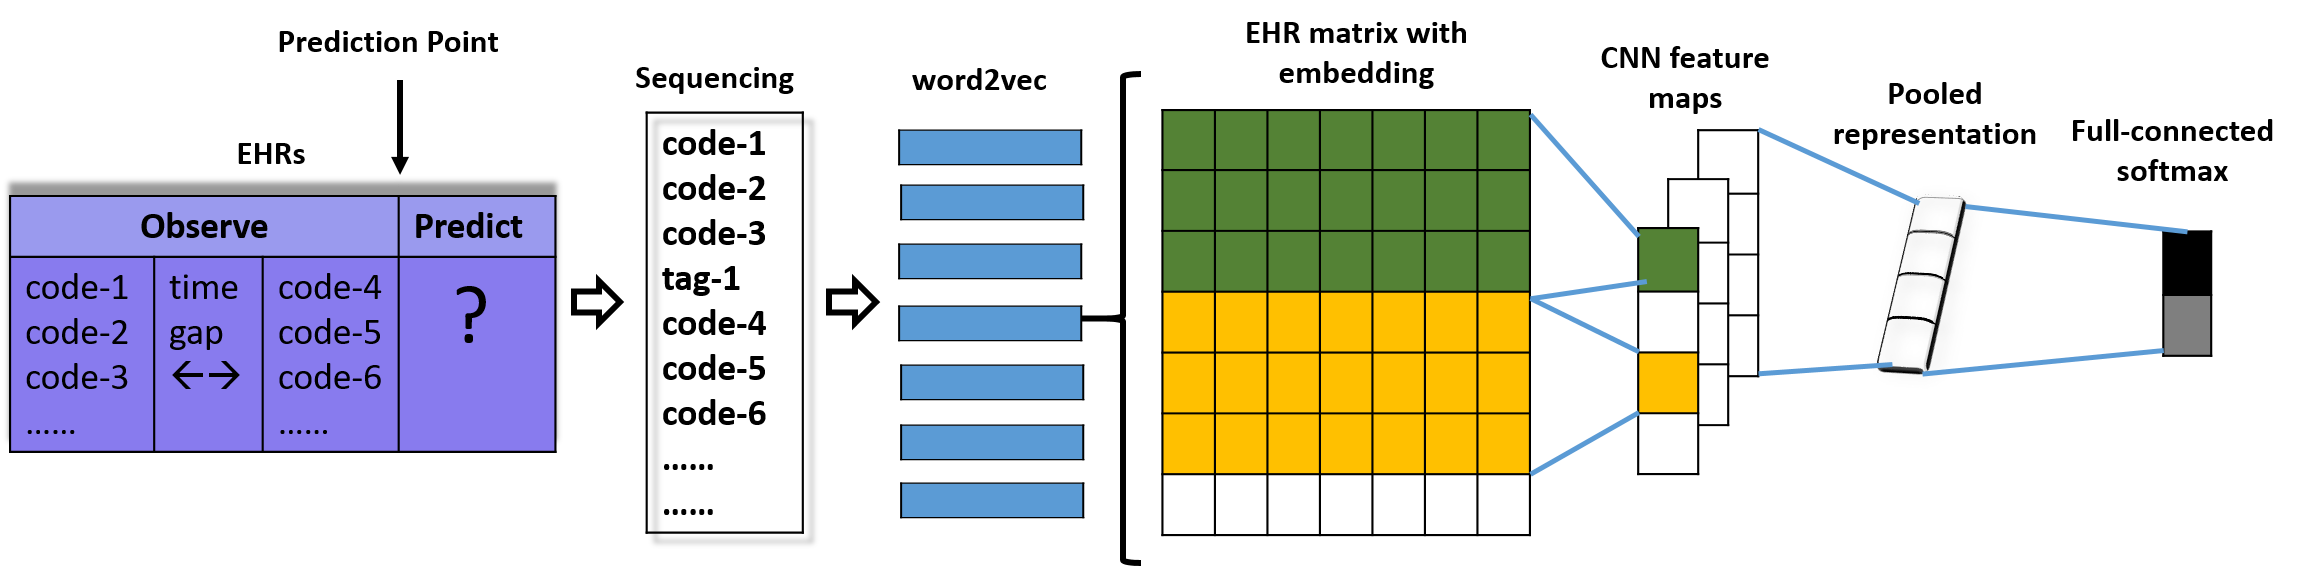
\includegraphics[width=6in]{CNNmodel} 
		\caption{Structure of Convolutional Neural Network Prediction Model}
		\label{fig:CNNmodel}
	\end{figure}
	
	
	\section{Implementation}
	\label{sec:exp}
	%\input{exp.tex}
	
	\subsection{Data Source}
	
	(Since we have not obtained access to the Sutter Health dataset yet, we will in the meantime give a description of the MIMIC-III dataset)
	
	\paragraph{}We utilized MIMIC-III v1.4 data set, which was released in September 2016.  There are 46520 patients and 651047 diagnosis events, 240095 procedures and 4156450 prescriptions. Each diagnosis event is associated with a hospital admission time, which is used to assign a sequential order to the ICD9 codes. Each procedure and prescription event are in forms of text names. 
	
	%(But I think we need to determine the cohort windows here?)
	
	
	\subsection{Implementation Details and Evaluation}
	
	\paragraph{}We will apply CNN to the word2vec embeddings to predict the diagnosis of HF. We take MIMIC-III data and train the Word2Vec model using all patients’ prescription, procedure, and diagnosis records, padded with appropriate time tags. We will then set the dimension of the embedding as X. In risk prediction stage, we will set the observation window and prediction window as 2000? days and 90? days, respectively. In order to train a more robust model, we will only keep patients that have a minimum of 50? records in their observation window. We will subsequently identify all the case group with patients diagnosed with any type of HF (ICD9 codes with 428.XX). We found that only a portion of patients can be categorized as case group. To keep the case and control classes balanced, for each patient in case group, we will randomly choose two control patients from those without HF diagnosis code. The resulting size of case and control group will be XXX and XXX. In MIMIC-III data, diagnosis records are not directly timestamped. We will use the admission time of the hospital stay during which diagnosis was given as the timestamp of each diagnosis. We set 6 filters with size from 2 to 7 in the convolutional layer followed by one pooling layer and two fully connected layers. We use the rectified linear unit (ReLU) activation function in convolution layer and fully connected layers. We use RMSprop as the optimizer. The CNN model is implemented in Keras with Tensorflow as the backend.
	
	We randomly separate the data set by 7:1:2 into the training set, validation set, and test set and the performance of the prediction will be evaluated in the test set.
	
	After CNN is trained, we will extract the output of the pooling layer concatenated with demographic features as the representation of each patient. We will use a PCA? (t-SNE?) algorithm to reduce the dimensionality of patient representation to two dimensions and visualize different groups in case and control patients. We will perform clustering algorithms on the case group and evaluate clusters by comparing the subgroups vs. the groups we identified as different types of HF such as rEF, pEF, or some other novel phenotypes. (tentative, if identifiable)
	
	
	\section{Results}
	\label{sec:interpret}
	%\input{interpret.tex}
	
	\subsection{Risk Prediction}
	Table \ref{tab:predResults} shows the summary of results of the prediction with different models. 
	
\begin{table}
	\vspace*{3mm}
	\caption{Summary of prediction results}
	\label{tab:predResults}
	\vspace*{2mm}
	\centering
	\begin{tabular}{c|ccc}
		\hline
		Place & Holder & for & Table\\ 
		\hline
		&  &  & \\
		\hline
	\end{tabular}
\end{table}
	
	%Overall our models achieved comparable results as previous studies, showing robustness of word2Vec and CNN in terms of predicting heart failure diagnosis in 90 days or later. XX model shows slightly better performance over others, indicating XXX.
	
	\subsection{Interpretation of Patient Representation and Phenotyping}
	
	Figure 2 shows control and case groups in form of patient representation extracted from CNN, dimension reduced by t-SNE.
	
	*Figure 2*
	
	Figure 3 shows subgroups in case group using clustered upon the patient representation and groups identified with two types of EF. 
	
	*Figure 3*
	
	Table \ref{tab:clusterDiagMed} shows some most common diagnosis and medications in different case subgroups identified by CNN.
	
\begin{table}
	\vspace*{3mm}
	\caption{Common diagnoses and medications for each cluster}
	\label{tab:clusterDiagMed}
	\vspace*{2mm}
	\centering
	\begin{tabular}{c|ccc}
		\hline
		Place & Holder & for & Table\\ 
		\hline
		&  &  & \\
		\hline
	\end{tabular}
\end{table}
	
	
	
	\section{Discussion}
	\label{sec:conclusion}
	%\input{conclusion.tex}
	
	Discussion of results will go here.
	
	
	%\section{Outline}
	%\label{sec:outline}
	%\input{outline.tex}
	
	%ACKNOWLEDGMENTS are optional
	%\section{Acknowledgments}
	%This work was supported by the National Science Foundation, award IIS- \#1418511 and CCF-\#1533768, Children's Healthcare of Atlanta, CDC I-SMILE project, Google Faculty Award,  AWS Research Award, Microsoft Azure Research Award and UCB.
	
	
	\section{References}
	\label{sec:references}
	\begin{enumerate}
		\item Alba AC, Agoritsas T, Jankowski M, Courvoisier D, Walter SD, Guyatt GH, Ross HJ. “Risk Prediction Models for Mortality in Ambulatory Patients With Heart Failure. A Systematic Review.” Circ Heart Failure. 2013. 6(5):881–9.
		
		\item Austin PC, Tu JV, Ho JE, Levy D, Lee DS. “Using methods from the data-mining and machine-learning literature for disease classification and prediction: a case study examining classification of heart failure subtypes.” Journal of clinical epidemiology. 2013. 66(4):398-407.
		
		\item Che Z, Cheng Y, Sun Z, Liu Y. “Exploiting Convolutional Neural Network for Risk Prediction with Medical Feature Embedding.” arXiv preprint arXiv:1701.07474. 2017.
		
		\item Che Z, Dale D, Li W, Bahadori MT, Liu Y. “Deep Computational Phenotyping.” KDD. 2015.
		
		\item Choi E, Bahadori MT, Kulas JA, Schuetz A, Steward WF, Sun J. “RETAIN: An Interpretable Predictive Model for Healthcare using Reverse Time Attention Mechanism.” NIPS. 2016.
		
		\item Choi E, Bahadori MT, Schuetz A, Stewart WF, Sun J. “Doctor AI: Predicting Clinical Events via Recurrent Neural Networks.” Proceedings of Machine Learning for Healthcare. arXiv preprint arXiv:1511.05942, 2015.
		
		\item Choi E, Bahadori MT, Searles E, Coffey C, Sun J. “Multi-layer Representation Learning for Medical Concepts.” arXiv preprint arXiv:1602.05568. 2016.
		
		\item Heidenreich PA, Trogdon JG, Khavjou OA, Butler J, Dracup K, Ezekowitz MD. “Forecasting the future of cardiovascular disease in the United States: a policy statement from the American Heart Association. Circulation. 2011. 123(8):933–44.
		
		\item Jensen PB, Jensen LJ, Brunak S. “Mining electronic health records: towards better research applications and clinical care.” Nature Reviews Genetics, 2012. 13(6):395-405.
		
		\item Karpathy A, Toderici G, Shetty S, Leung T, Sukthankar R, Fei-Fei L. “Large-scale video classification with convolutional neural networks.” Proceedings of the IEEE conference on Computer Vision and Pattern Recognition. 2014. 1725-32.
		
		\item Kim, Yoon. "Convolutional neural networks for sentence classification." arXiv preprint arXiv:1408.5882 (2014).
		
		\item LeCun Y, Bengio Y, Hinton G. “Deep learning.” Nature. 2015. 521.
		
		\item Lindman BR. “The Diabetic Heart Failure with Preserved Ejection Fraction Phenotype: Is It Real and Is It Worth Targeting Therapeutically?” Circulation. 2017. 135:736-40.
		
		\item Lipton ZC, Kale DC, Elkan C, Wetzel R. “Learning to Diagnose with LSTM Recurrent Neural Networks.” ICLR. 2016.
		
		\item Marr B. “First FDA Approval For Clinical Cloud-Based Deep Learning In Healthcare.” Forbes. 20 Jan 2017. Web.
		
		\item Mikolov T, Sutskever I, Chen K, Corrado GS, Dean, J. “Distributed representations of words and phrases and their compositionality.” Advances in neural information processing systems. 2013. 3111-9.
		
		\item Mozaffarian D, Benjamin EJ, Go AS. on behalf of the American Heart Association Statistics Committee and Stroke Statistics Subcommittee. Heart disease and stroke statistics—2016 update: a report from the American Heart Association. Circulation. 2016. 133:e38-e360.
		
		\item Nguyen P, Tran T, Wickramasinghe N, Venkatesh S. “Deepr: A Convolutional Net for Medical Records.” IEEE journal of biomedical and health informatics. 2017. 21(1):22-30.
		
		\item Ross JS, Mulvey GK, Stauffer B, Patlolla V, Bernheim SM, Keenan PS, Krumholz HM. “Statistical models and patient predictors of readmission for heart failure: a systematic review.” Archives of internal medicine. 2008. 168(13):1371-1386.
		
		\item Smith DH, Johnson ES, Thorp, ML, Yang X, Petrik A, Platt RW, Crispell K. “Predicting poor outcomes in heart failure.” The Permanente Journal, 2011. 15(4), 4.
		
		\item Taslimitehrani V, Dong G, Pereira NL, Panahiazar M, Pathak J. “Developing EHR-driven heart failure risk prediction models using CPXR (Log) with the probabilistic loss function.” Journal of biomedical informatics. 2016. 60:260-269.
	\end{enumerate}
	
	
	%
	% The following two commands are all you need in the
	% initial runs of your .tex file to
	% produce the bibliography for the citations in your paper.
	%\bibliographystyle{abbrv}
	%\bibliography{med2vec}  % sigproc.bib is the name of the Bibliography in this case
	% You must have a proper ".bib" file
	%  and remember to run:
	% latex bibtex latex latex
	% to resolve all references
	%
	% ACM needs 'a single self-contained file'!
	%
	%APPENDICES are optional
	%\balancecolumns
\end{document}